\documentclass[conference]{IEEEtran}
%\documentclass[journal]{IEEEtran}

\usepackage{graphicx}
\newcommand{\ppv}{P_{pv}}
\newcommand{\pinv}{P_{inv}}

\title{Simulations of Efficiency Improvements using Measured Microgrid Data}

\begin{document}

\author{
\IEEEauthorblockN{Daniel Soto}
\IEEEauthorblockA{
The Earth Institute\\
Columbia University\\
New York, NY 10027}
\and
\IEEEauthorblockN{Vijay Modi}
\IEEEauthorblockA{
Department of Mechanical Engineering\\
Columbia, University\\
New York, NY  10027}
}

\maketitle

\begin{abstract}
Reaching unelectrified populations in the developing world
with distributed solar requires agressive cost optimization of
generation and storage.
Conventional solar generation architectures using photovoltaic
panels, sealed lead acid batteries, and inverters show room for
cost improvement.
Using data collected from photovoltaic microgrid users and simulations
we demonstrate potential cost reductions using alternate
technologies and architectures.
Reducing losses from power conversion could lower wholesale energy
costs by 20\% while improved battery chemistries could lower
costs by up to 50\%.
\end{abstract}

\section{Introduction}

The cost of renewable and distributed energy systems must be
optimized to sustainably provide electricity to the customers
beyond the reach of the grid.
Private energy service companies (ESCOs) may be able to supply power
where utilities have failed to reach.
However, as private companies, ESCOs will be especially sensitive
to the price of generation and the ability to collect
tariffs.
This constraint makes it necessary to optimize energy systems
for cost.
Since these systems are often paid for by the revenue collected
from electricity sales, these optimizations are important.
\cite{Lemaire-2011}
Our previous work has focused on the improved collection of
tariffs through mobile commerce and prepayment \cite{ICTD}.
This work will focus on potential cost reductions which allow
the same level of energy to be delivered for a lower total
investment and cost per kWh.

Our observations of electricity use in newly electrified villages
show usage patterns that are difficult to serve efficiently
with existing technology.
Our data show that villages whose primary electricity use is
lighting, television, and cell phone charging have wide variation
in power.
This work presents opportunities for efficiency and therefore
cost reduction in the areas of power conversion and storage.
These recommendations are based on data collected from customers
who have recently been provided with a near-grid-quality
electrical connection and are paying for that power on a
per kilowatt-hour basis.
There are many optimizations of system size in the literature
\cite{optimizations}.
This work adds to the literature by considering the effects
of the time of day of usage and the efficiencies of commonly
used inverters and batteries.
Conventional inverters cannot service this variation in power
at a consistent efficiency.
This decrease in efficiency leads to an increase in both
generation and storage costs.

Two approaches to mitigation of this load variation exist,
the first is scheduling or addition of loads that smooth consumption.
The second approach is developing a power converter architecture
that is less sensitive to the variation in loads.
We present data addressing the first approach, where two of our
sites have added freezers.
Our microgrid data and simulations show that these daytime loads
can increase the cost-effectiveness of a microgrid.
For the second approach we model the cost reductions possible
for a hypothetical inverter that has a more constant efficiency
across all loads in its operating range.
This could be achieved through multiple inverters with
different operating regimes or future improvements in inverter
technology.
Although modest gains are available through load management or
inverter efficiency, larger efficiency
gains are possible as battery technologies improve.
In addition to modeling effects of inverter efficiency and load
variation, we model the system cost using existing sealed lead acid
battery technology and promising Lithium and Lead Carbon
technologies.
The improved efficiency and lifetimes of these emerging technologies
can significantly reduce the cost of off-grid electricity
where per kWh costs are currently dominated by the need
for storage.


\section{Microgrid and Data Description}

The simulations in this paper will use data collected from
Mali.
This section describes the solar photovoltaic microgrid
systems that this data is taken from.
It will also describe some of the notable features in the data.

\subsection{Data collection}
We have installed 17 solar photovoltaic microgrid systems
with remote connectivity using Short Message Service (SMS)
over the Global System for Mobile Communications (GSM) networks
in Mali and Uganda as described in \cite{ICTD}.
These systems allow customers to purchase bundles of
electricity in advance of use either through a scratch card and
cell phone purchase or through a tablet device.
Each of these systems consists of a 1.4 kWp array of photovoltaic
panels with a 48 V, 360 Ah battery bank.
An MPPT charge controller handles battery charging and a
750 W inverter supplies the microgrid with 50 Hz, 220 V power.
Up to 20 customers are connected to these systems in a star
topology where each customer has a dedicated wire to the
central facility.
Each customer is metered by a commercially available device that
allows for energy measurement and reporting and a switch to
automatically connect or disconnect the consumer.
In addition to communication regarding the purchase of power,
these systems send data on an hourly basis to a central server
using SMS messages.
Data is collected on the energy consumption of each household
as well as the AC energy consumption of the entire system.
From the solar controller, we measure and store hourly information
on the solar energy delivered to the system and the battery
voltage.
This data stream allows us to observe consumer usage and payment
behavior.

\subsection{Timeseries Description}
These messages allow us to create a database of timeseries
information from the customers.
In this paper we focus on data from a few microgrids in
Mali that are representative of the demand from rural residential
customers.
In these residential settings, the most common appliances are
light bulbs, cellphones, and televisions.
Consequently, the peak power is consumed in the evening
as shown in Figure \ref{two-bulb-profile}.
Customers in these microgrids were provided with two light bulbs
as part of the installation.
In Figure \ref{two-bulb-profile}, the two bands in the evening show
that usage clusters around these values.
Most of the customers have little or no usage during the day time.

\begin{figure}[h]
\begin{center}
% 93bc6d og ghtc2012.py
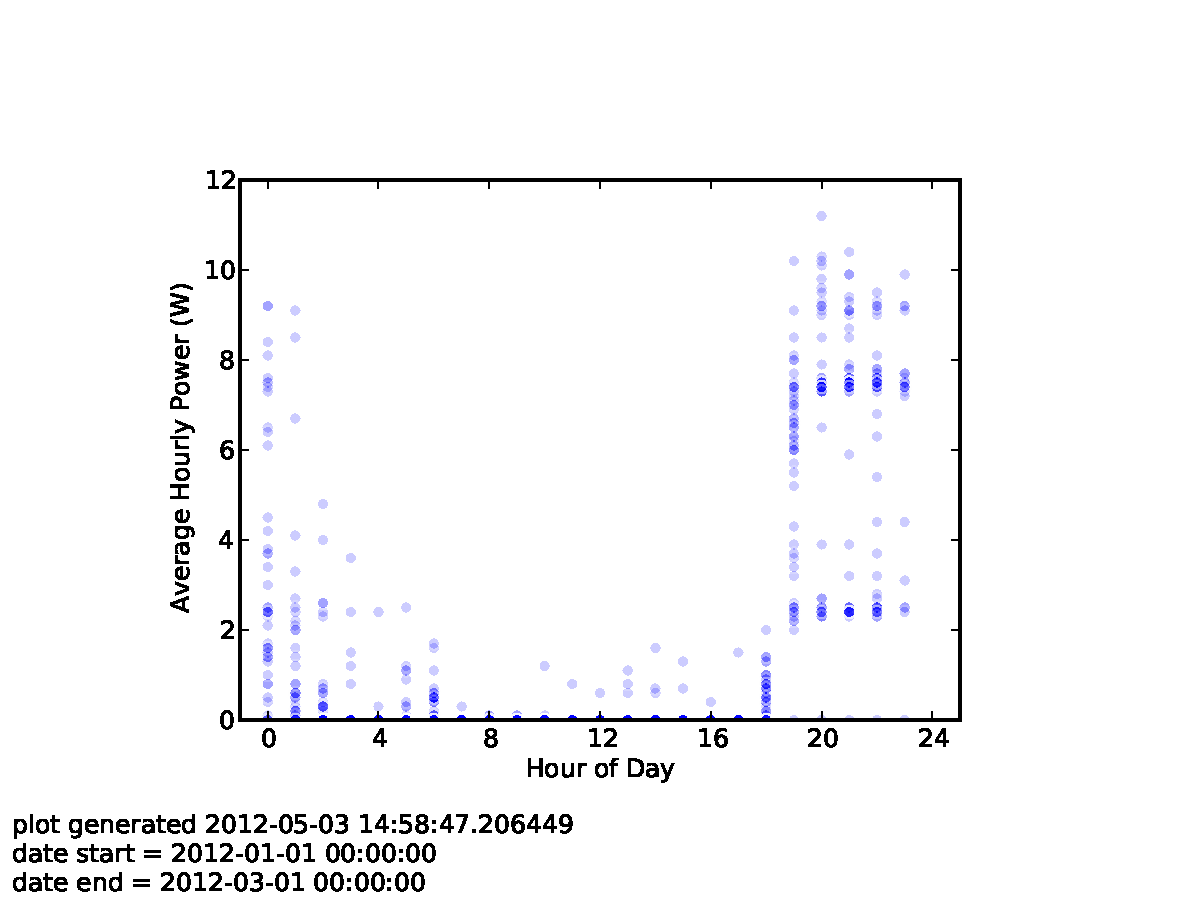
\includegraphics[trim = 0.7in 0.8in 0.7in 1.1in, clip, width=\columnwidth]
{figures/two_bulb_profile.pdf}
\end{center}
\caption{Customer exhibiting two bulb lighting load.
Each data point is the hourly load for a single day.
Multiple days are superimposed.
Points are transparent so that frequent measurements appear darker.
This customer displays two common evening power levels corresponding
to the use of one or two lightbulbs.
This not that this customer has very small power use during the day.}
\label{two-bulb-profile}
\end{figure}

The addition of daytime loads can reduce the percentage of variation
in demand.
In two microgrid systems, freezers have been installed that customers are using to
sell ice or frozen drinks.
These freezers significantly increase the daytime load on the system.
The hourly profile for the household using this freezer
is shown in Figure \ref{freezer}.
These freezers draw a much larger amount of power than the
typical lighting load and have a lower variation when measured
on an hourly basis.

\begin{figure}[]
\begin{center}
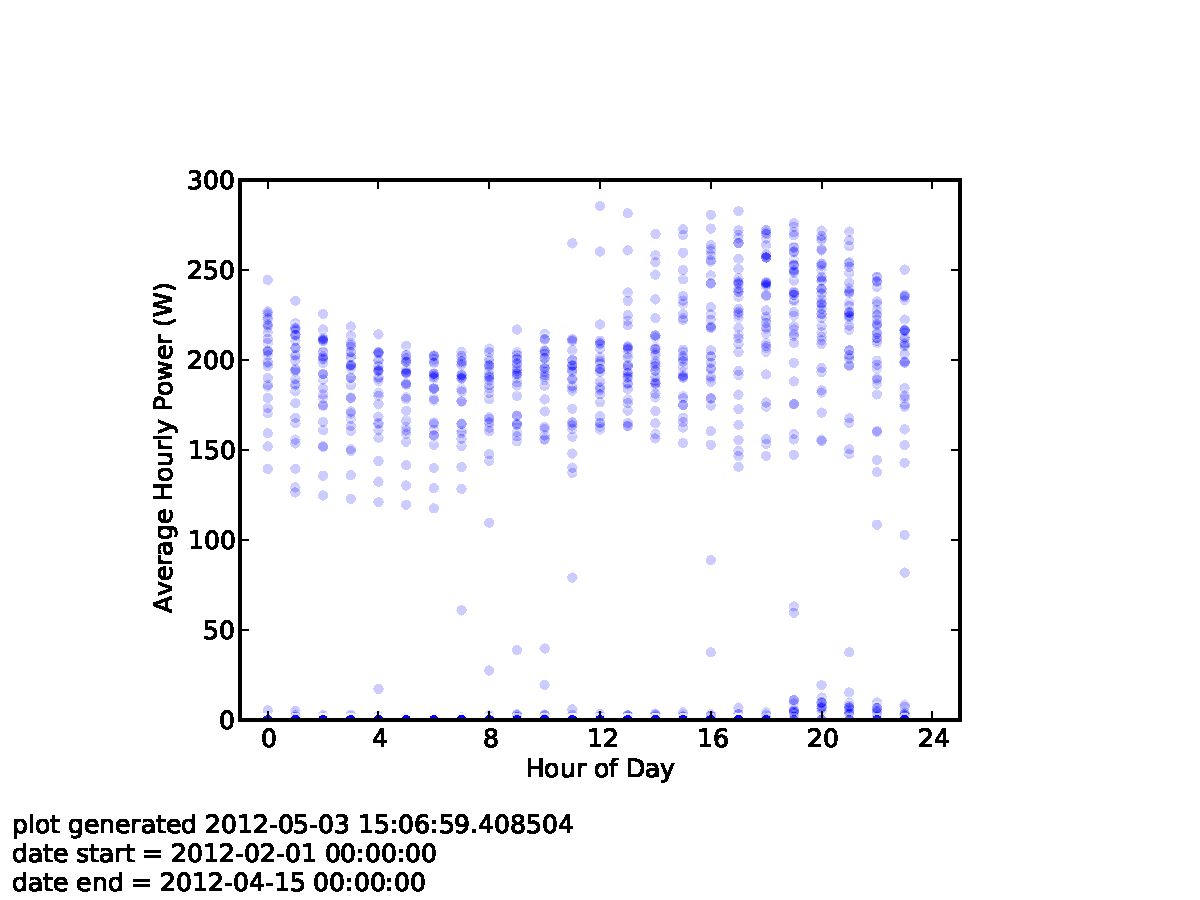
\includegraphics[trim = 0.7in 0.8in 0.7in 1.1in, clip, width=\columnwidth]
{figures/freezer_profile.pdf}
\end{center}
\caption{Circuit with freezer.
Each data point is the hourly load for a single day.
The absolute variation in power is still significant but the
ratio between high and low use is lower.}
\label{freezer}
\end{figure}

\subsection{Load Duration Curves}

To visualize the variation in load, we use a load-duration-curve
to summarize the load demanded by the microgrid.
If we sort the hourly power demand over a long time period, we
construct a load duration curve \cite{REEPS}.
A load-duration curve (Figure \ref{two_ldc}) shows this variation.
In the microgrid that does not have a freezer, the most common
power level is less than 50W, which is well below the peak
efficiency of the inverter.
For the system that does have a freezer, the system spends the bulk
of its time consuming on the order of 200W, which is much closer
to the peak efficiency operating point of the inverter.
The inverter is sized so that the maximum customer load is safely
accommodated by the inverter.
However, there is a substantial efficiency penalty for operating the
inverter below the optimal point.

We can express these loads in terms of the capacity factor,
where the capacity factor is relative to the rated output
of the inverter.
Systems with high power variability will lose efficiency since
the system will often be operated outside of the range of
peak efficiency.

\begin{figure}[h]
\begin{center}
% og ghtc2012.py 07d761 plot_two_ldc()
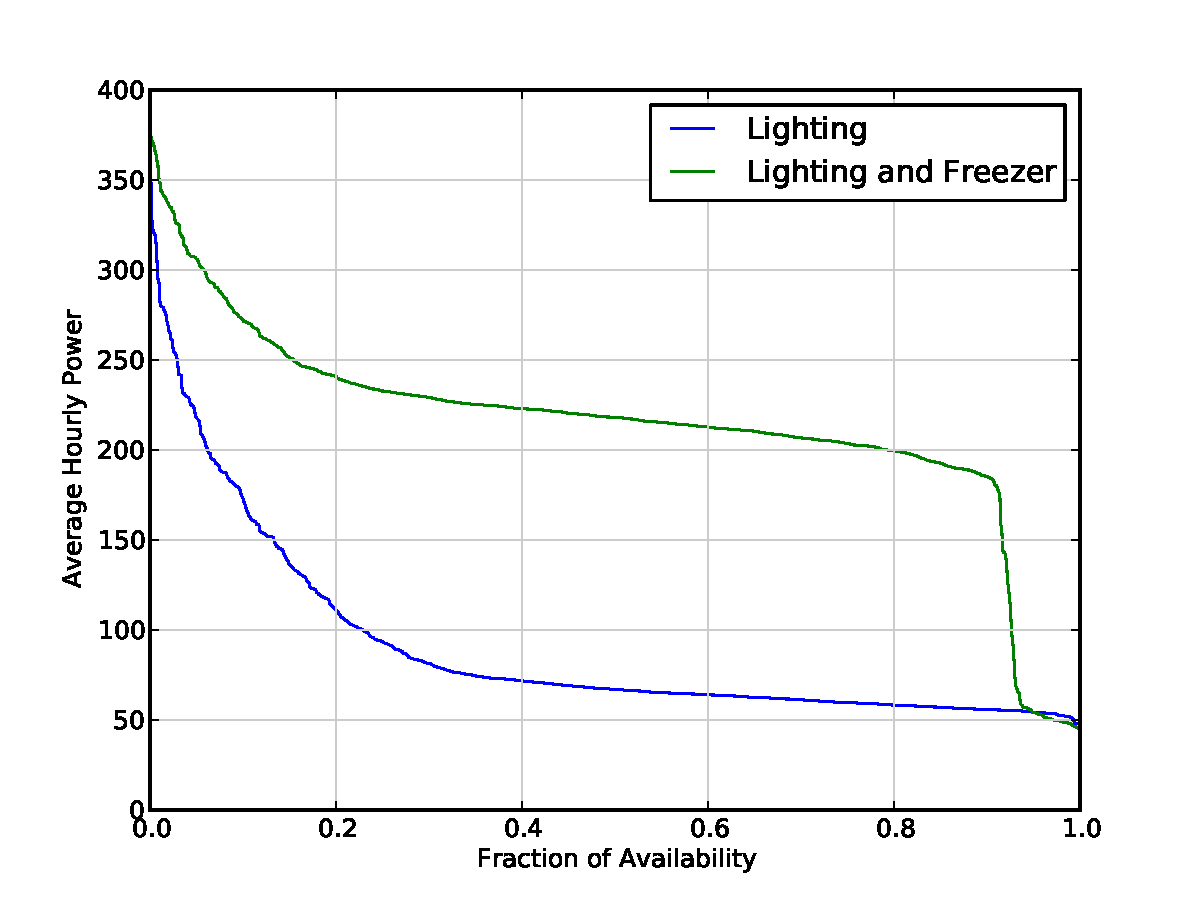
\includegraphics[trim = 0.0in 0.2in 0.0in 0.5in, clip, width=\columnwidth]{figures/two_ldc.pdf}
\end{center}
\caption{Load duration curve for two typical microgrid systems,
including metering, computing, and computation.
Inverter and charge controller consumption is not included.
One system includes a significant daytime refrigeration load,
while the other does not.
}
\label{two_ldc}
\end{figure}

\subsection{Overall System Efficiency}

We can estimate an overall system efficiency from the
system-wide usage data and information from the solar
controller on photovoltaic energy generation.
This estimate of the overall efficiency of the system
is defined as DC power delivered by solar
power controller divided by the AC power delivered to the system
to power both the system electronics and the user loads.
Our data shows that as the capacity factor of the inverter
increases, the overall system efficiency improves.
In sites with a freezer and therefore considerable daily load,
the inverter capacity factor is approximately 30\% and
we see an overall efficiency of 0.88--0.90.
In a lighting only site, with much less daily load, the capacity
factor is less than 15\% and the overall efficiency
is less than 0.70.
The large variations in loads exhibited by these customers prompted
us to investigate the impact on system efficiency that these
variations in loads are causing.

\section{Simulation Description}

We examine the effect of load variation and alternate technologies
on the size and cost of the system by creating an
energy simulation of the system.
The simulation finds the minimum panel size and battery capacity
that will meet the demand assuming clear-sky radiation.
This model is intended to allow comparisons between systems and
load profiles rather than provide accurate guidance for system
sizes over a typical meteorological year.
The simulation takes as input the hourly load profile from a
set of either real or hypothetical customers.
The model then uses a series of assumptions on battery and solar
panel parameters to calculate the power and storage at each hour.
The battery is considered to be a simple energy storage device
with perfect efficiency during charging and an efficiency of
$\eta_B$ on discharge.
We can calculate the energy in the battery in discrete time
steps according to the following equation.
%
$$ E_B(t+\Delta t) = E_B(t)
                   + P_{charge} \cdot \Delta t
                   - \frac{P_{discharge} \cdot \Delta t}{\eta_B}
                   $$
%
Where $P_{charge}$ is the power flow when the photovoltaic
production is greater than the inverter demand and
$P_{discharge}$ is the power flow when the inverter demand
is greater than the photovoltaic power available.
They are given by the following equations.
%
$$ P_{charge} = \left\{
			  \begin{array}{rl}
			  0 & \pinv > \ppv \\
			  \ppv - \pinv & \pinv < \ppv
			  \end{array}
			  \right. $$
%
$$ P_{discharge} = \left\{
			  \begin{array}{rl}
			  \pinv - \ppv & \pinv > \ppv \\
			  0 & \pinv < \ppv
			  \end{array}
			  \right. $$
%
Where $\pinv$ is the DC power demanded by the inverter and
$\ppv$ is the power being delivered by the charge controller.
$\pinv$ is calculated using the efficiency
of the inverter as a function of AC load according to
$$ \pinv = \frac{P_{AC}}{\eta_{inv}(P_{AC})} $$
%
Where $P_{AC}$ is the hourly power demanded by the consumers of the microgrid.

The difference equation is run in a loop where the
panel size in the model is adjusted until the energy remaining
in the battery at the end of the simulation is equal to the
energy at the start of the simulation.
The minimum battery size is then the peak-to-peak variation
of the battery energy time series.
A time series trace is shown in Figure \ref{simulation}.
Once the simulation finds a solution where the starting and final
storage are equal, the model outputs the minimum battery size
to meet the storage need at 100\% depth of discharge and the
minimum solar panel size to meet the demand.
Based on panel size and battery size output along with the
assumptions on panel cost and battery cost and life, the model
predicts the net present value (NPV) of the system over the
life of the system.
In this model we use a 7\% discount factor and a 20-year time
horizon.
The battery, inverter, and panel assumptions for these simulations are listed in
Table \ref{table_battery_assumptions},
Table \ref{tbl_inverter_assumptions},
and Table \ref{table_panel_assumptions}.

\begin{figure}[h]
\begin{center}
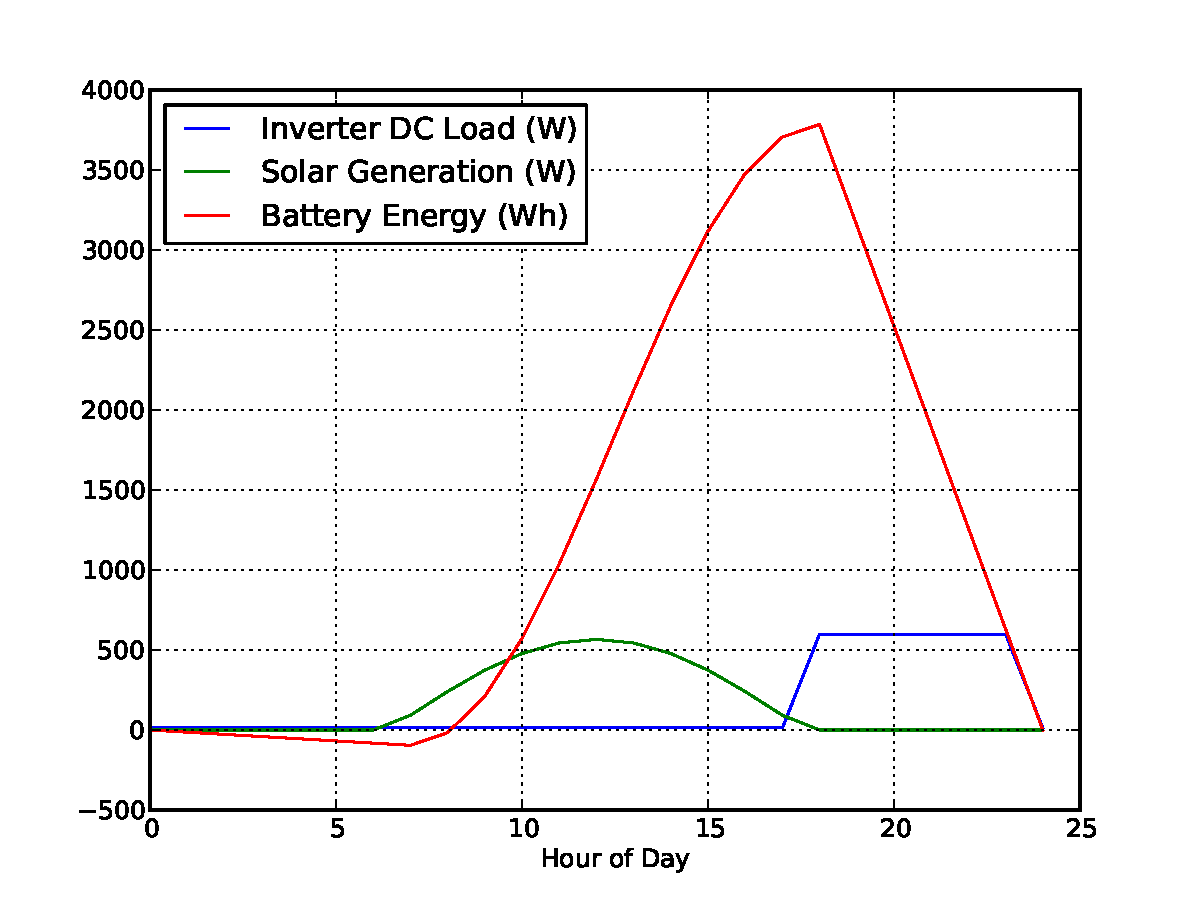
\includegraphics[trim = 0.0in 0.2in 0.0in 0.5in, clip, width=\columnwidth]{figures/simulation.pdf}
\end{center}
\caption{
Time series of simulation.
The DC load of the inverter is plotted along with the solar generation
as a function of hour.
The solar panel size is adjusted until the battery energy at the end
of the simulation is the same as the start value.
}
\label{simulation}
\end{figure}

\begin{table*}
\centering
\begin{tabular}{ c c c c c }
Battery Chemistry            & Initial Cost & Lifetime & Optimal & Storage    \\
                             & (USD/kWh)    & (yr)     & DOD     & Efficiency \\
Sealed Lead Acid (SLA)       & \$140        & 2        &  50\%   & 75\%       \\
Lithium Iron Phosphate (LFP) & \$1000       & 6        & 100\%   & 95\%       \\
Lead Carbon (PbC)            & \$140        & 6        &  50\%   & 75\%       \\
\end{tabular}
\caption{Battery Assumptions for Modeling.}
\label{table_battery_assumptions}
\end{table*}

\begin{table}
\centering
\begin{tabular}{ c c }
Rated Power               & 750 W \\
Peak Efficiency           & 94\%  \\
No-load Power Consumption & 13 W  \\
\end{tabular}
\caption{Inverter Assumptions for Modeling.}
\label{tbl_inverter_assumptions}
\end{table}


\begin{table}
\centering
\begin{tabular}{ c c }
Panel Efficiency & 13.5\%   \\
Panel Latitude   & 14 N     \\
Panel Cost       & \$1/W    \\
Panel Lifetime   & 20 years \\
\end{tabular}
\caption{Solar Panel Assumptions for Modeling.}
\label{table_panel_assumptions}
\end{table}


\section{Calculation Results and Discussion}

The simulation results compare the performance of hypothetical
systems to the baseline system and report potential improvements.

\subsection{Baseline System}
The simulated baseline system is based on the system we have
installed in the field.
The inverter efficiency for this baseline system is shown in Figure
\ref{inverter_curves} as the ``Baseline'' curve.
The battery used in the baseline system is the Sealed Lead Acid
battery in Table \ref{table_battery_assumptions}.
The solar panel assumptions used in the baseline and all other
simulations are listed in Table \ref{table_panel_assumptions}.
This baseline system is used for comparison against the
improvements discussed below.

\begin{figure}[]
\begin{center}
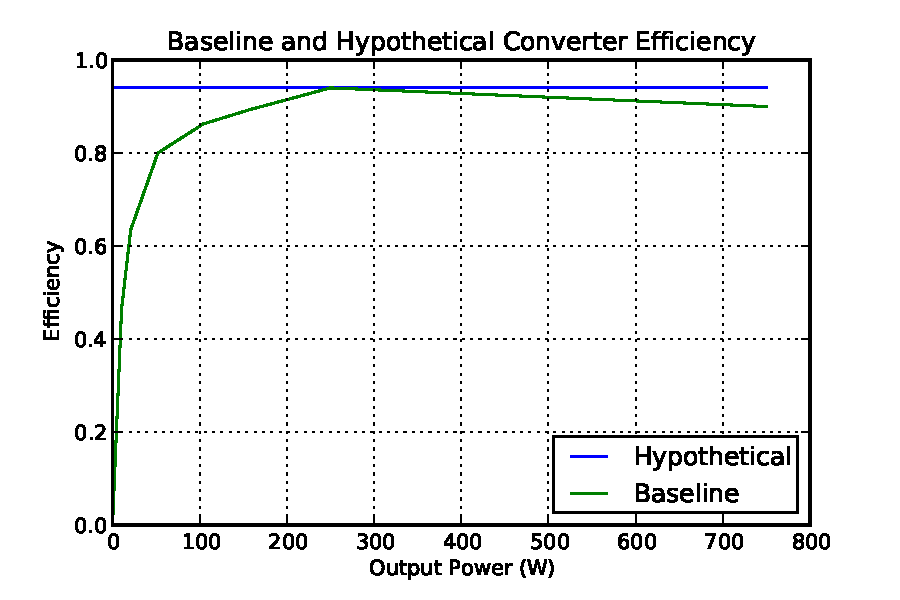
\includegraphics[width=\columnwidth]{figures/inverter_curves.pdf}
\end{center}
\caption{Efficiency curves for baseline and proposed system.}
\label{inverter_curves}
\end{figure}

\subsection{Impact of load shape}

The storage and generation necessary to service a given daily
amount of energy can vary depending on what time of day
that energy is delivered.
To demonstrate the effect of the time of day that power
is consumed on the generation and storage capacity of the system,
we calculate the panel and battery size for five loads with
the same total daily energy but occurring at different times of day.
We define a ``Night'' load that has the entire day's load
occurring between 6pm and midnight.
We also define a ``Day'' load that occurs between 9am and 3pm
and a ``Constant'' load that is evenly spread across the entire day.

In addition to these three hypothetical loads, we also use loads
representative of the measured customer loads at our microgrids.
The ``Lighting'' village load uses a representative day from one of the
village microgrids and has a small constant load and a large
nighttime load.
The ``Freezer'' village load is from one of our microgrids using a freezer
to provide ice for sale.

We calculate the minimum generation and storage for each
of these five loads.
Table \ref{tbl_baseline} shows a detailed output of the panel and
battery sizes and NPV costs over an assumed 20 year lifetime
which demonstrate the variability of panel size and battery
size with the type of load.
Figure \ref{fig_baseline}
shows these results in terms of an estimated cost of delivered
electricity.
Only in the ``Day'' load is the generation cost a significant
fraction of the total cost.
There are variations in the size and price of the panel
necessary to meet the load, but the cost impact is small
compared to the storage costs.
For the other loads, the storage cost is dominant.
Note that we do not include balance of system costs or
distribution costs since these will be much less sensitive
to these load types.
The lowest total cost is delivered for the ``Day'' load
since there is very little storage necessary.
The highest total cost is incurred for the ``Night'' load since
the storage demand is the greatest.


\begin{figure}[]
\begin{center}
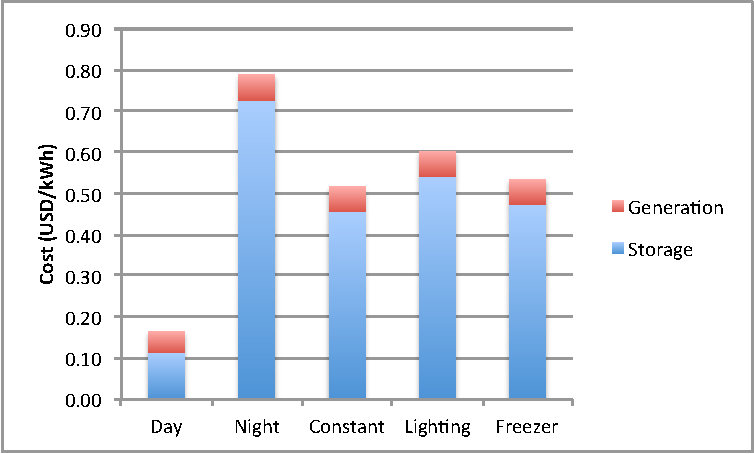
\includegraphics[width=\columnwidth]{figures/baseline.pdf}
\end{center}
\caption{Cost of electricity for different load profiles using Baseline
inverter and battery system and hypothetical and measured loads.}
\label{fig_baseline}
\end{figure}

\begin{table*}
\centering
\begin{tabular}{c c c c c}
Configuration & Panel Capacity & Minimum Battery & Battery NPV & Solar NPV \\
              & (kWp)          & Size (kWh)      & (USD)       & (USD)     \\
\hline
% village_simulation 845102 table_2()
typical day lead acid        & 0.59 & 0.76 & 1306 & 595 \\
typical night lead acid      & 0.74 & 4.92 & 8421 & 738 \\
typical continuous lead acid & 0.70 & 3.08 & 5281 & 704 \\
typical village lead acid    & 0.73 & 3.66 & 6270 & 727 \\
\end{tabular}
\caption{Impact of load time-of-day on system size.
Loads are normalized to 3.0 kWh per day.}
\label{tbl_baseline}
\end{table*}

\subsection{Inverter Efficiency}

In a system with a wide variation in power levels the inverter can
be a significant loss of power.
A typical inverter is inefficient at loads below its
preferred operating point.
If the load is usually close to this high efficiency
point, the lower efficiencies at low power are not important.
If however, as we observe, there is a high variability
in the power output where daytime loads are very small
but evening loads are greater, this inefficiency can have
a significant impact.
If the system is run inefficiently during the daytime, the inefficiency
burden only impacts the amount of generation capacity needed.
If the system is run inefficiently during the evening, both the
generation and the storage costs are affected, multiplying the
penalty.
Late-night and early morning cellphone charging and vampire
loads can cause this inefficiency.
To demonstrate this effect, we run our simulation with
a hypothetical power conversion device that has an
efficiency equal to the peak efficiency of the baseline
inverter at any power level.
Table \ref{table_inverter} shows the detailed simulation
results.
The increase in inverter efficiency reduces the generation
and storage needed for four of the five load types.
The reductions in battery NPV and solar NPV could offset the
additional cost of a dedicated low-power inverter with a
cross-over circuit for when the load requires the high-power inverter.
Figure \ref{fig_inverter}
shows the impact on delivered price for the five loads we
consider in this work.

\begin{figure}[]
\begin{center}
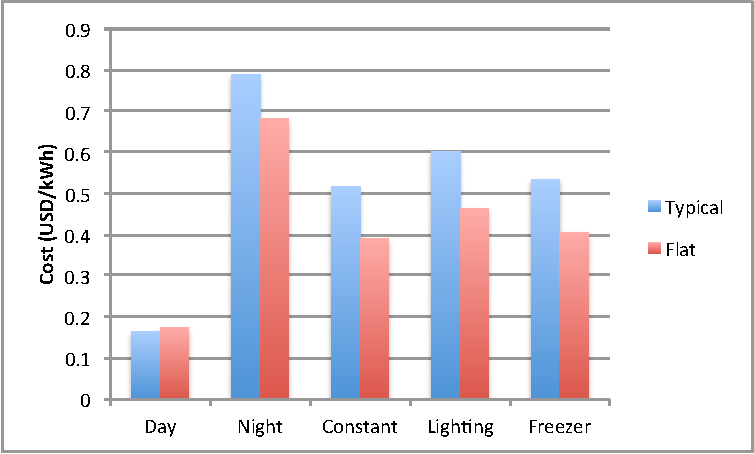
\includegraphics[width=\columnwidth]{figures/inverter.pdf}
\end{center}
\caption{Cost of electricity for different load profiles using Baseline
inverter and battery system and hypothetical and measured loads.}
\label{fig_inverter}
\end{figure}

\begin{table*}
\centering
\begin{tabular}{c c c c c}
Load Type     & Panel Capacity & Minimum Battery & Battery NPV & Solar NPV \\
              & (kWp)          & Size (kWh)      & (USD)       & (USD)     \\
\hline
% table_inverter
% 2012-05-09 07:42
% 3e30fa
Day        & 0.50 & 0.88 & 1509 & 498 \\
Night      & 0.62 & 4.26 & 7289 & 621 \\
Continuous & 0.53 & 2.33 & 3993 & 532 \\
Lighting   & 0.55 & 2.81 & 4819 & 553 \\
Freezer    & 0.53 & 2.44 & 4176 & 532 \\

\end{tabular}
\caption{Impact of inverter non-ideality on system size.
Simulations use single-point efficiency inverter and
SLA battery.
Loads are normalized to 3.0 kWh daily.}
\label{table_inverter}
\end{table*}

\subsection{Battery Chemistry}

The largest potential for cost reduction can come from improved
battery technologies.
Current lead acid technologies lasting 500--1000 cycles, must be
replaced every 2--3 years depending on the environment.
In terms of initial cost, batteries are comparable to the photovoltaic
panel cost but their frequent replacement makes the storage cost
dominant over the lifetime of the system.
Differences in allowable depth of discharge (DOD) and the round-trip
energy efficiency of the battery can also influence the lifetime
cost of the storage.

New battery chemistries could reduce the fraction of investment
that goes toward storage of electricity.
The incumbent battery technology is sealed lead acid (SLA).
Emerging technologies of interest are Lithium Iron Phosphate
(LFP) and Lead Carbon (PbC).

Relative to SLA batteries, LFP batteries
have better cycle life, higher specific cost, and better
turnaround efficiency.
PbC batteries are not yet mature but promise improved cycle
life and likely similar specific cost and turnaround
efficiency.
The assumptions for the battery types in the simulation
are found in Table \ref{table_battery_assumptions}.

The initial battery cost is given by
%
$$ C_B = E_{storage} \frac{1}{\eta_B} \frac{1}{DOD_{optimal}} c_B $$
%
Where $E_{storage}$ is the storage necessary, $\eta_B$ is the
round trip energy efficiency, $DOD_{optimal}$ is the desired
operating point of the battery for long life, and $c_B$ is the
initial cost of the battery per kWh.
A very important metric however is the life cycle cost of the
battery replacement which depends on the cycle life of the battery.

The life cycle cost is the net present value (NPV) of the
initial and replacement battery expenditures over the life
of the system.
In this simulation we use a 7\% discount factor and a 20-year
system lifetime.
The baseline inverter is used in these simulations.

We simulate the impact of these on system size and total cost
in Table \ref{table_battery}.
Figure \ref{fig_battery} shows the impact of battery type on
the per kWh cost of electricity.
For the case of typical village data, the lifetime cost of
lead acid and LFP are similar.
If LFP costs reach the \$500/kWh cost targets mentioned in
the context of electric vehicles, these batteries will
be a clear choice.
If PbC batteries are able to maintain their cost while
improving cycle life, they will provide a clear improvement
in the life-cycle cost.
Both of these battery simulations are speculative but given
the dominance of storage costs in these systems, attention
to emerging battery technologies is worthwhile.

\begin{figure}[]
\begin{center}
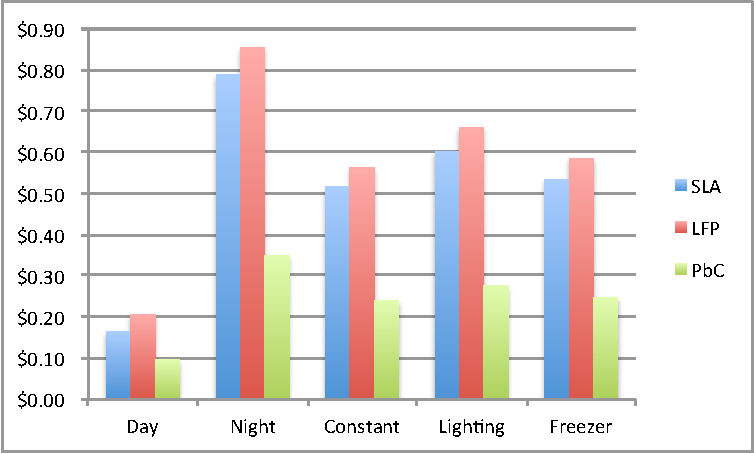
\includegraphics[width=\columnwidth]{figures/battery.pdf}
\end{center}
\caption{Cost of electricity for different battery chemistries.}
\label{fig_battery}
\end{figure}


\begin{table*}[!t]
\centering
\begin{tabular}{ c c c c c c }
Load Type & Battery & Panel Capacity & Minimum Battery & Battery NPV & Solar NPV \\
          & Type    & (kWp)          & Size (kWh)      & (USD)       & (USD)     \\
\hline
% table_5()
% 2012-05-09 07:29
% git commit a49634
%Day        & SLA & 0.59 & 0.76 & 1306 & 595 \\
%Day        & LFP & 0.57 & 0.76 & 1824 & 566 \\
%Day        & PbC & 0.59 & 0.76 & 514  & 595 \\
%
%Night      & SLA & 0.74 & 4.92 & 8421 & 738 \\
%Night      & LFP & 0.59 & 3.88 & 9338 & 587 \\
%Night      & PbC & 0.74 & 4.92 & 3312 & 738 \\
%
%Continuous & SLA & 0.70 & 3.08 & 5281 & 704 \\
%Continuous & LFP & 0.61 & 2.46 & 5931 & 609 \\
%Continuous & PbC & 0.70 & 3.08 & 2077 & 704 \\

Lighting    & SLA & 0.73 & 3.66 & 6270 & 727 \\
Lighting    & LFP & 0.62 & 2.93 & 7043 & 615 \\
Lighting    & PbC & 0.73 & 3.66 & 2466 & 727 \\

Freezer     & SLA & 0.70 & 3.21 & 5500 & 703 \\
Freezer     & LFP & 0.61 & 2.57 & 6186 & 606 \\
Freezer     & PbC & 0.70 & 3.21 & 2163 & 703 \\

\end{tabular}
\caption{Simulation results for battery chemistries.
Net present value is calculated at 7\% over 20 year
time horizon.}
\label{table_battery}
\end{table*}


\section{Discussion / Future Work}
While the simulation results discussed are speculative,
we believe that experimentation in this regime is important.
We have emphasized supply and generation optimizations in
this work but would like to point out the importance of
efficient appliances.
Efficient appliances allow services to be delivered at the
lowest possible price.
Our microgrids use LED lighting to achieve the best cost for
lighting in terms of price per kilolumen-hour delivered.
The televisions that we have observed in these microgrids
have been inefficient cathode ray tube (CRT) televisions
with power loads of over 50W.
The price per hour of entertainment could be lowered by providing
more efficient liquid crystal display (LCD) televisions.
In addition to increasing the amount of services that the consumer
can gain for a given amount, these reductions in demand
reduce the amount of generation and storage needed.
These demand side improvements can lower the system size and
deliver the services people want for less power.

In addition to improving the efficiency of the end-uses of
the system, efficiency can be gained by some architectural
choices.
Casillas and Kammen show that the introduction of meters
to a rural microgrid lowered usage \cite{Casillas-2010}.
Thomas and coauthors estimate that LED lighting using DC
building circuits lower costs relative to AC connected
LED circuits \cite{EdisonRevisited}.
Since all loads in our residential areas are DC loads,
AC inverter costs and inefficiencies may be unnecessary.
The IEEE/Sirona Haiti Rural Electric Project
uses only
DC circuitry and DC-only laptop charging stations
are being developed for schools \cite{Hosman}.
The addition of meters to a grid installation or the use of a
DC only architecture could also lower overall life-cycle cost
for new installations.


\section{Summary}
Hourly demand data for newly electrified communities has been gathered.
We find that improving no-load and low-load power consumption of the
inverter can reduce storage and generation needs and lower the cost
of electricity 20\% for many load types.
Future battery chemistry types have the potential to deliver 50\%
reductions in the wholesale cost of electricity to consumers.


%\section{Acknowledgements}



\begin{thebibliography}{1}

\bibitem{optimizations}
Z Wissem, K Gueorgui, K H\'edi,
Modeling and techinical--economic optimization of an autonomous
photovoltaic system,
Energy, Vol. 37, 2012 pp. 263-272
(doi:10.1016/j.energy.2011.11.036)

\bibitem{ICTD}
D.~Soto, M. Basinger, S. Rodriguez, E. Adkins, R. Menon,
I. Willig, N. Owczarek, V. Modi,
``A Prepaid Architecture for Solar Electricity Delivery In Rural Areas''
\textit{Proceedings of the Fifth International Conference on Information
and Communication Technologies and Development,}
(ICTD2012)
(doi:10.1145/2160673.2160691)

\bibitem{REEPS}
G.~Masters,
"Renewable and Efficient Electric Power Systems",
Wiley Interscience,
2004

\bibitem{Lemaire-2011}
X. Lemaire,
``Off-grid electrification with solar home systems:
The experience of a fee-for-service concession in South Africa'',
Energy for Sustainable Development,
Vol 15, pp. 277--283, 2011,
(doi:10.1016/j.esd.2011.07.005)

\bibitem{Casillas-2010}
C. Casillas, D. Kammen,
``The delivery of low-cost, low-carbon rural energy services'',
Energy Policy,
Vol. 39, pp. 4520--4528, 2011,
(doi:10.1016/j.enpol.2011.04.018)

\bibitem{EdisonRevisited}
B.A. Thomas, I. L. Azevedo, G. Morgan,
``Edison Revisited:
Should we use DC circuits for lighting in commercial buildings?'',
Energy Policy,
Vol. 45, pp. 399--411, 2012
(doi:10.1016/j.enpol.2012.02.048)

\bibitem{Hosman}
http://theinstitute.ieee.org/benefits/humanitarian-efforts/keeping-laptops-alive-in-haiti
\end{thebibliography}

\end{document}

%---------------------------------------------------------------------------%
%---------------------------------------------------------------------------%
%---------------------------------------------------------------------------%
%---------------------------------------------------------------------------%
%---------------------------------------------------------------------------%
%---------------------------------------------------------------------------%
%---------------------------------------------------------------------------%
%---------------------------------------------------------------------------%
%---------------------------------------------------------------------------%
%---------------------------------------------------------------------------%
%---------------------------------------------------------------------------%
%---------------------------------------------------------------------------%


